The main goal in this project is to detect and identify balls. There are different approaches to solving this problem. One approach is to concentrate on solving both problems at once by identifying balls directly and thereby also implicitly detecting them. Other approaches, like the one used in this project, performs the detection first to determine the regions of interest and then extracts further data from the regions for use in the identification process.

The advantage of the former is that the computation can be done in one pass. Features that are used to identify the balls, can in this way also be used in the detection process. This results in a more robust detection because that a correctly identified ball implies a correct detection.

The advantage of the latter is that the identification algorithm only has to be applied to the detected areas and thereby reducing the computational complexity.

\section{Solution Ideas}

\subsection{Template Matching}
By constructing templates that represents the different ways a ball can be turned, e.g. with the number facing up, the stripe turned different ways, template matching can be applied to identify balls on the table. This method will do detection and matching at the same time and thereby utilize the information contained in the template, concerning color and shape, to both find an accurate matching position and at the same time identify the ball which will be equal to the equivalent template.

Using this method requires that a sufficient number of templates are created to cover the possible ways that a ball is turned. Templates are created by either sampling balls in many different positions, or generating them using the knowledge of color and looks of a ball. Problems arise when similar colored balls are in close proximity, as this will create matches in positions between the balls.

The template punishes textural differences between the template and the area being matched. This means that for a template to give a good match, the ball has to face the same way in the template as in the matching area.
balls. 

The method also has high complexity for the reason that each template has to be matched against the entire table.

Experiments with matching a simple one-colored template against the balls proved inaccurate. The color distribution in a ball is not narrow enough to provide a good match against a single colored template. The number area and pixels with high intensity caused by reflections causes the template to match in positions away from the ball center.

\subsection{Histogram Backprojection}
Histograms extracted from training data are backprojected against the entire image of the pool table. This is done by computing the histogram inside a mask in every image position, and then assigning a score to the position by measuring the difference between the sampled and model training histogram.\cite{learningOpenCV}

This process is similar to the template matching described above, but instead of taking structure of the image into account the, i.e. where the different colors are located inside the circular mask, this method evaluates the distribution of the colors regardless of structure.
\begin{figure}[htpb]
  \centering
  \subfloat[Good match]{\label{fig:backProjectGood}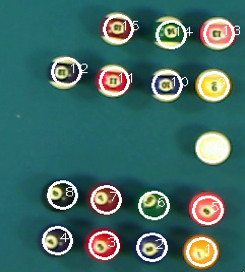
\includegraphics[width=0.48\textwidth]{images/backprojectGood.png}}
  \quad           
  \subfloat[Bad match]{\label{fig:backProjectBad}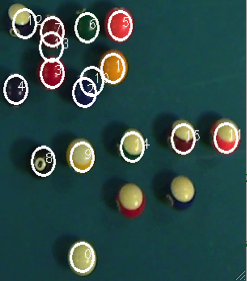
\includegraphics[width=0.48\textwidth]{images/backprojectBad.png}}
   \caption{Results of the backprojection method. Labeled white circles indicate identified balls.}
  \label{fig:backprojectResults}
\end{figure}
Backprojection has difficulties in dealing with the different ways a ball can face. Depending on the way the ball is facing, the distribution is going to change based on color differences in the surface and the amount of white area that is visible. This results in large differences between the measured and the model distribution, when they are compared in strict sense, i.e. bin by bin. If e.g. the two histograms are equal, but one is shifted, the output will be that they are different. A less strict comparison where, e.g. only the mean is used to measure similarity is preferred.

Figure \ref{fig:backprojectResults} shows results of experiments of backprojection methods. The model histograms that results in a good match against \ref{fig:backProjectGood}, has problems in \ref{fig:backProjectBad} where the balls are facing differently.

\subsection{BLOB Analysis}
The uniform color of the table cloth can be utilized to apply a threshold to the image resulting in BLOBs representing ball locations. The BLOBs can be separated using morphology operations to separate balls in close proximity. The center position of BLOBs or a feature like the bounding circle, can be used to mark the center point of a ball. Pixels that are inside a BLOB is extracted for further processing to identify the ball.
\begin{figure}[htpb]
  \centering
  \subfloat[Original]{\label{fig:blobAnalBefore}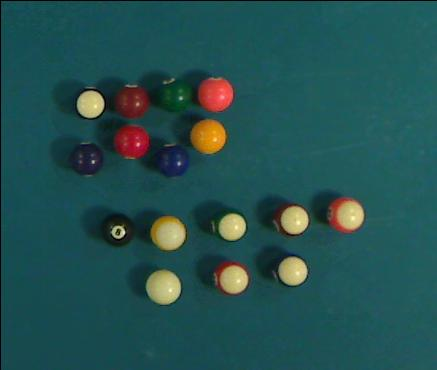
\includegraphics[width=0.48\textwidth]{images/blobAnalBefore}}
  \quad           
  \subfloat[Segmented using threshold, eroded]{\label{fig:blobAnalAfter}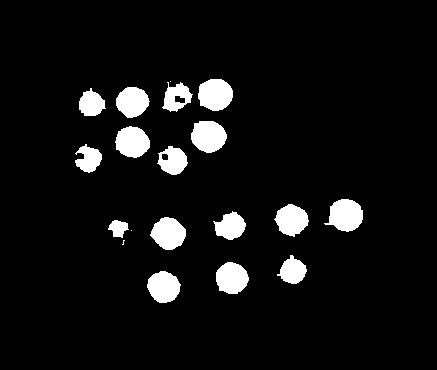
\includegraphics[width=0.48\textwidth]{images/blobAnalAfter}}
   \caption{Example of problems with using BLOB analysis.}
  \label{fig:blobAnal}
\end{figure}
As will be mentioned later in this section, this kind of segmentation is useful for reducing the ROI, but using the pixels in a BLOB can cause problems. If the area represented by the BLOB does not include all pixels of a ball or includes pixels from other balls, problems arise in detection and identification. This situation is in figure {\ref:blobAnal}. This happens frequently when balls are laying too close to produce separate BLOBs, but instead ends up as one large BLOB containing pixels from several balls.

\subsection{Chosen Solution: Ball Probability Estimation}
The solution used in this project uses the two-step process by first detecting ball positions and thereafter identifying the detected balls.

The detected positions must be precise to gain the optimal working conditions for the identifier. A ball position that is slightly shifted will result in a ball region that contains pixels that does not belong to the ball. This will make it harder for the identifier to identify the ball, and it will become even harder if the region intersects other balls, because the region will then become a mix of two different balls. 

The detection is performed by estimating the probability that a ball is present at every position inside a ROI on the table. The positions in the image having the highest probabilities are considered ball locations and can be passed on to the identifier.

The identification process can be separated into two steps: determining if the ball is striped and determining the color of the ball. The ball is considered striped if the ratio between white and colored pixels are above a certain level (see section \ref{sec:analballs}). The color is determined by comparing the distribution of the color in the detected position with known training data.